%%%%%%%%%%%%%%%%%%%%%%%%%%%%%%%%%%%%%%%%%
% Beamer Presentation
% LaTeX Template
% Version 1.0 (10/11/12)
%
% This template has been downloaded from:
% http://www.LaTeXTemplates.com
%
% License:
% CC BY-NC-SA 3.0 (http://creativecommons.org/licenses/by-nc-sa/3.0/)
%
%%%%%%%%%%%%%%%%%%%%%%%%%%%%


%----------------------------------------------------------------------------------------
%	PACKAGES AND THEMES
%----------------------------------------------------------------------------------------

%\documentclass[10pt]{beamer}
\documentclass[]{beamer}



\DeclareMathOperator*{\argmin}{arg\,min}


%%%%%%%%%%%%%

\usepackage{hyperref}


\newcommand{\bi}{\begin{itemize}}
\newcommand{\ei}{\end{itemize}}
\newcommand{\m}{\item}
\newcommand{\be}{\begin{enumerate}}
\newcommand{\ee}{\end{enumerate}}
\newcommand{\al}{\alert}
\newcommand{\ul}{\underline}


\mode<presentation> {

% The Beamer class comes with a number of default slide themes
% which change the colors and layouts of slides. Below this is a list
% of all the themes, uncomment each in turn to see what they look like.

%\usetheme{default}
%\usetheme{AnnArbor}
%\usetheme{Antibes}
%\usetheme{Bergen}
%\usetheme{Berkeley}
%\usetheme{Berlin}
%\usetheme{Boadilla}
%\usetheme{CambridgeUS}
%\usetheme{Copenhagen}
%\usetheme{Darmstadt}
%\usetheme{Dresden}
\usetheme{Frankfurt}
%\usetheme{Goettingen}
%\usetheme{Hannover}
%\usetheme{Ilmenau}
%\usetheme{JuanLesPins}
%\usetheme{Luebeck}
%\usetheme{Madrid}
%\usetheme{Malmoe}
%\usetheme{Marburg}
%\usetheme{Montpellier}
%\usetheme{PaloAlto}
%\usetheme{Pittsburgh}
%\usetheme{Rochester}
%\usetheme{Singapore}
%\usetheme{Szeged}
%\usetheme{Warsaw}

% As well as themes, the Beamer class has a number of color themes
% for any slide theme. Uncomment each of these in turn to see how it
% changes the colors of your current slide theme.

%\usecolortheme{albatross}
%\usecolortheme{beaver}
%\usecolortheme{beetle}
%\usecolortheme{crane}
%\usecolortheme{dolphin}
%\usecolortheme{dove}
%\usecolortheme{fly}
%\usecolortheme{lily}
%\usecolortheme{orchid}
%\usecolortheme{rose}
%\usecolortheme{seagull}
%\usecolortheme{seahorse}
%\usecolortheme{whale}
%\usecolortheme{wolverine}

%\setbeamertemplate{footline} % To remove the footer line in all slides uncomment this line
%\setbeamertemplate{footline}[page number] % To replace the footer line in all slides with a simple slide count uncomment this line

%\setbeamertemplate{navigation symbols}{} % To remove the navigation symbols from the bottom of all slides uncomment this line
}


%\setbeamertemplate{headline}
%{%
% \begin{beamercolorbox}{section in head/foot}
%\vskip1pt\insertnavigation{\textwidth}{}{}\vskip2pt
%  \end{beamercolorbox}
%}

\setbeamercolor{section in head/foot}{bg=lightgray} %set the top navigation bar background color
\setbeamertemplate{footline}[frame number] % set frame page number only
\usepackage{appendixnumberbeamer} % total will not include appendix frame numbers 

\beamertemplatenavigationsymbolsempty



\usepackage{graphicx} % Allows including images
% graphicx also allows for resizebox
% graphicx also allows for \scalebox
\usepackage{caption}
\usepackage{subcaption} % packgage for subcaption in subfigures
% The subfig and subcaption packages can not be used in cooperation with each other. Instead, you can usecaption package with subfig to add some flavor to the captions and subcaptions
\usepackage{bm} % make bold math symbols
\usefonttheme{professionalfonts}
%\usepackage{newtxtext,newtxmath} % for professional fond to load a Times Roman clone
\usepackage{tabularx} % extra features for tabular environment
\usepackage{booktabs} % Allows the use of \toprule, \midrule and \bottomrule in tables
\usepackage{adjustbox} % allows adjustbox
\usepackage{amsmath}  
\usepackage{amsfonts}
\usepackage{hyperref} % package for hyper link

% the following hypersetup makes link blue
\hypersetup{
  colorlinks   = true, %Colours links instead of ugly boxes
  urlcolor     = blue, %Colour for external hyperlinks
  linkcolor    = blue, %Colour of internal links
  citecolor   = blue %Colour of citations
}


\usepackage{float} % make the table H effective
\restylefloat{table}
\usepackage{color, colortbl}
\usepackage{booktabs} % package for tex professional table
\usepackage{mathtools} % package for \coloneqq
\usepackage{multirow} % multirow for intuition page.

% make pdf dark mode
%\usepackage{xcolor}
%\pagecolor[rgb]{0,0,0} %black
%\color[rgb]{0.5,0.5,0.5} %grey

\usepackage{pifont}% http://ctan.org/pkg/pifont
\newcommand{\cmark}{\ding{51}}%
\newcommand{\xmark}{\ding{55}}%



\usepackage{tikz} % graph in latex
\usetikzlibrary{positioning,arrows.meta} %tikz diagram
\usepackage{pgfplots}
\pgfplotsset{compat=newest} %this setting allow node to go to the correct place
\usepgfplotslibrary{fillbetween}

% use the tikz external library to cache tikz drawings
\usetikzlibrary{external}
\tikzexternalize[prefix=tikz/,optimize command away=\includepdf]


%\bibliography{bibliography}
%\usepackage[american]{babel}
%\usepackage{csquotes}
%\usepackage[style=apa]{biblatex}
%\DeclareLanguageMapping{american}{american-apa}
%\addbibresource{References.bib}

\usepackage{natbib} % package for citation


%\usepackage{subfigure} % subfigure package
%\captionsetup[subfigure]{labelformat=empty}
% The subfig and subcaption packages can not be used in cooperation with each other. Instead, you can usecaption package with subfig to add some flavor to the captions and subcaptions

%\usepackage{natbib} % package for citation

% define a comment line that does nothing to hide content
\newcommand{\comment}[1]{}
\newcommand{\lnb}[1]{%
  \ln\left(#1\right)%
}
\renewcommand{\baselinestretch}{1.0} %  scales the default interline space to 1.0 its default value. 

% define a comment that can scale the equation 
\newcommand\scalemath[2]{\scalebox{#1}{\mbox{\ensuremath{\displaystyle #2}}}}

%----------------------------------------------------------------------------------------
%	TITLE PAGE
%----------------------------------------------------------------------------------------

\title[Governance and Non-Fungible Tokens]{\huge{Governance and Non-Fungible Tokens} \\
\vspace{6mm}
\small{MGT 4074 Fintech \& Crypto Tokens, Fall 2025}
} % The short title appears at the bottom of every slide, the full title is only on the title page


%\subtitle{Presentation to Shanghai International Studies University}


\author[Joseph Hall]{Joseph Hall} % Your name
\institute[GT]{Georgia Institute of Technology} % Your institution as it will appear on the bottom of every slide, may be shorthand to save space
 % Your institution for the title page
 % Your email address
 
\date{October 13, 2025} 
 % Date, can be changed to a custom date if without date



%---------------------------------------------------------------------------
\begin{document}

\newcolumntype{d}[1]{D{.}{.}{#1}}


\begin{frame}
\titlepage % Print the title page as the first slide
\end{frame}


%----------------------------------------------------------------------------------------

%	PRESENTATION SLIDES
%----------------------------------------------------------------------------------------

%-----------------------------------------------



%---------------------------------------------------------------------
%---------------------------------------------------------------------
%\section*{Introduction}
% When I comment the introduction section, fewer sections show up in navigation
%---------------------------------------------------------------------
%---------------------------------------------------------------------



\begin{frame}{In Praise of Ponzis}

\textbf{Q}: What is an \emph{Ponzi Scheme}?  \\ \pause 
\textbf{A}: A plan to pay early investors high returns using later investors' principal while performing \ul{no real investment.} 
\bi 
\m In a finite world, this plan must fail eventually. \pause 
\ei 
\textbf{Q}: Well then why does Dror Poleg praise them? \\ \pause 
\textbf{A}: Two reasons: 
\bi 
\m The story of the scheme itself may achieve such notoriety that its memory becomes an object of value in and of itself (like Bitcoin) 
\m Ponzi-\emph{like} (not Ponzi per se) economics may become a dominant force in a future digital economy: early adopters can become investors and marketers simultaneously \pause 
\ei 
Note that \textbf{Social Security} is literally a Ponzi Scheme.

\end{frame}


\begin{frame}{When Dror wrote this essay}

\begin{center}
    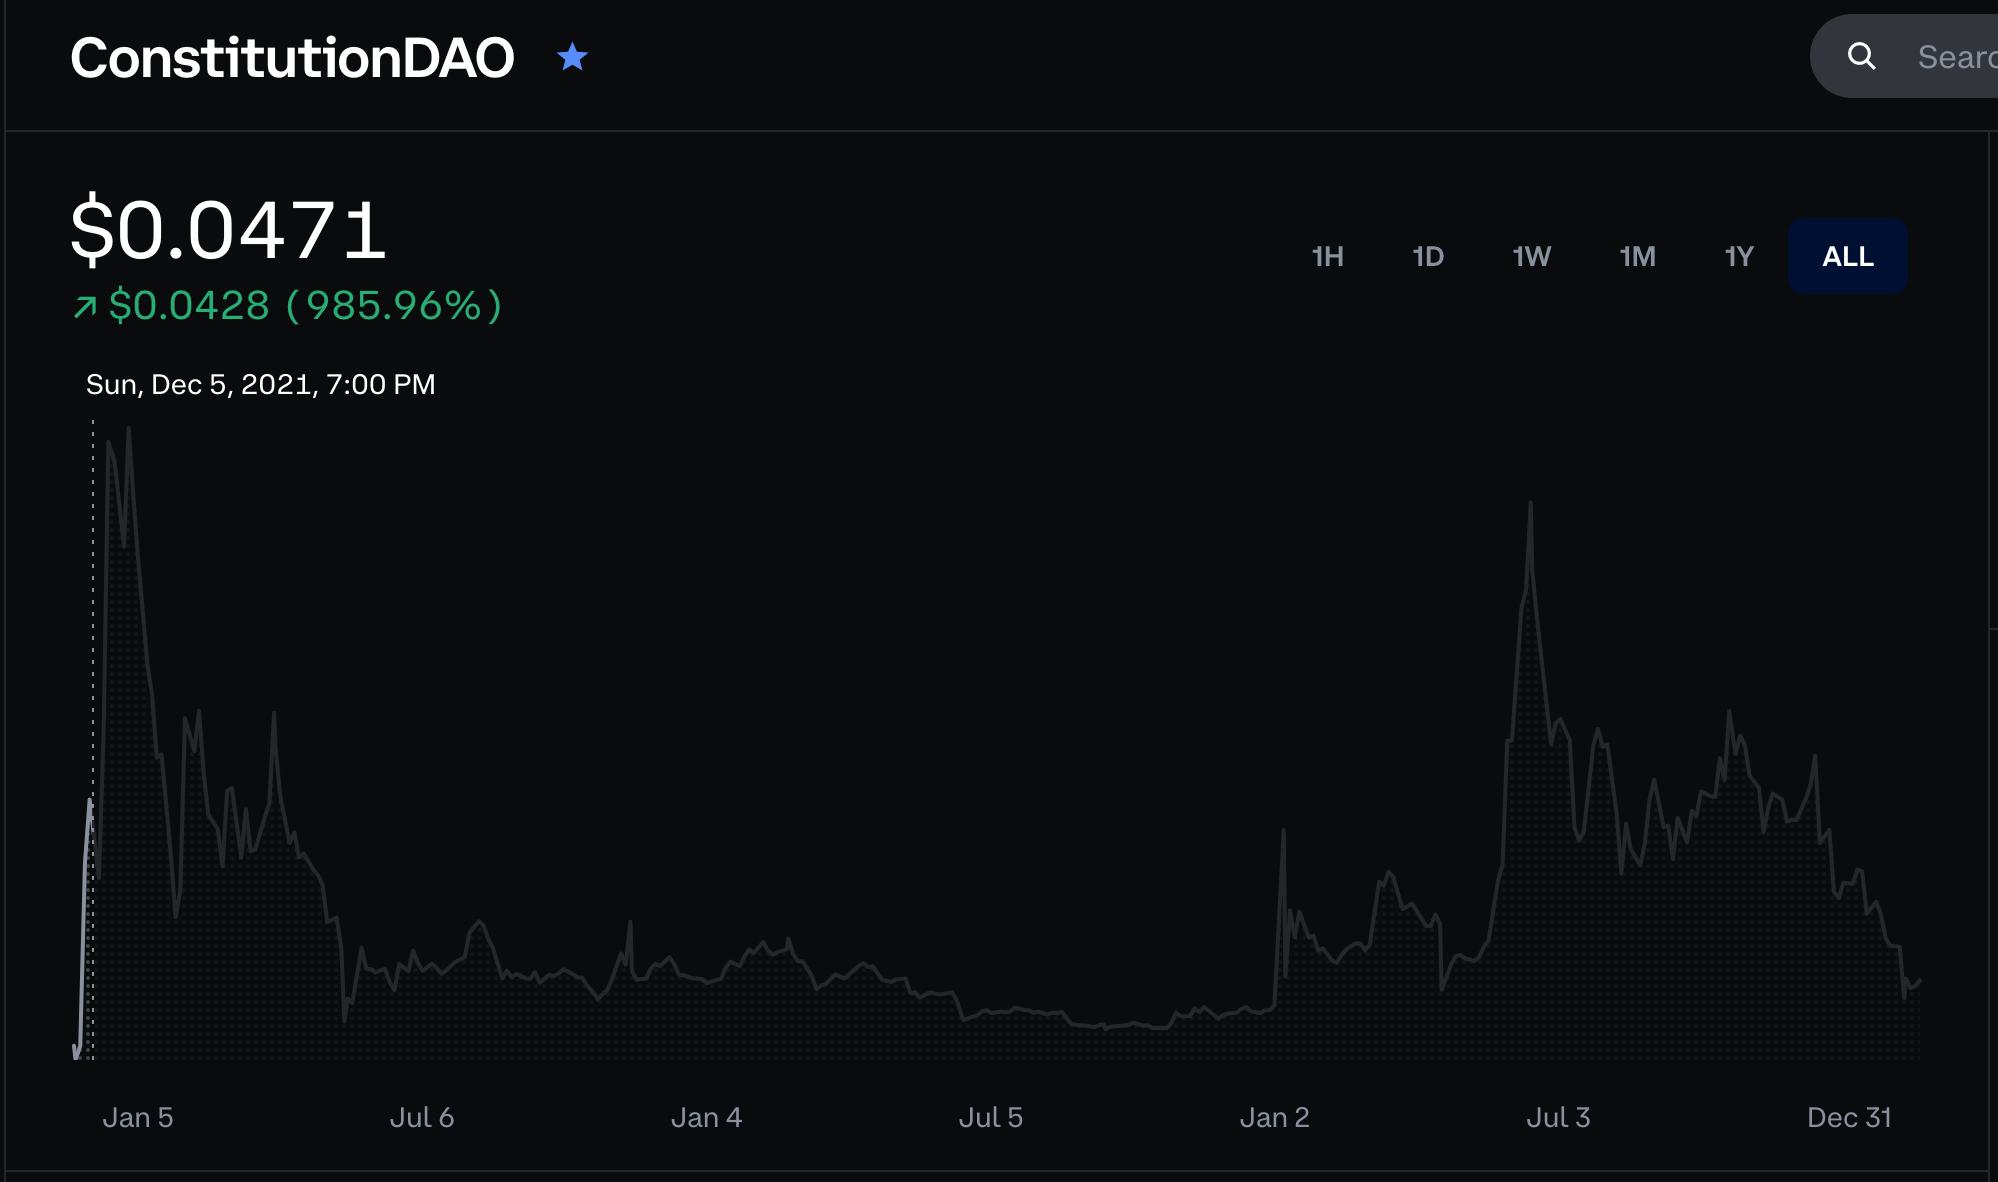
\includegraphics[width = \textwidth]{Screenshot 2025-02-13 at 4.22.37 PM.png}
\end{center}

    
\end{frame}

\begin{frame}{Since}

\begin{center}
    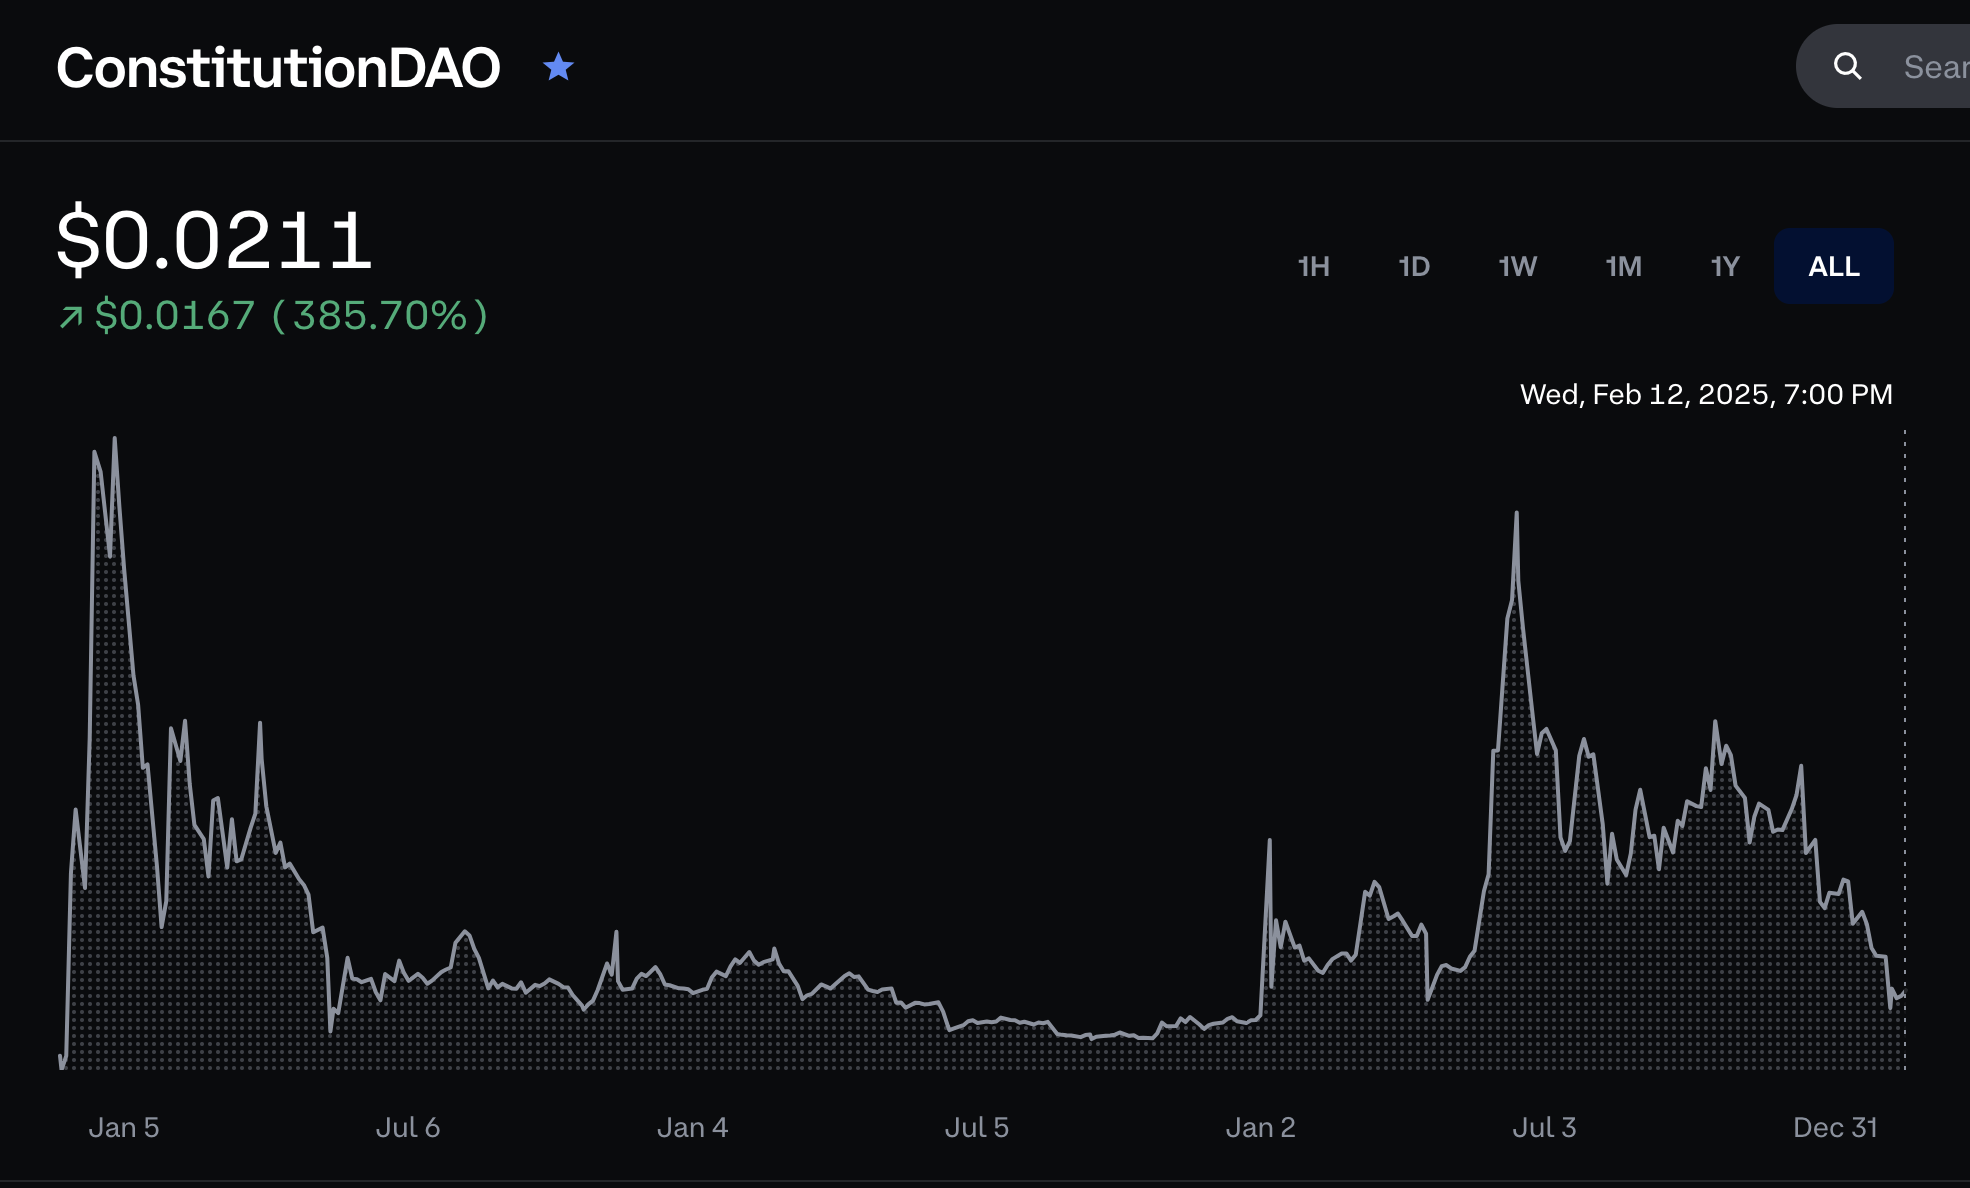
\includegraphics[width = \textwidth]{Screenshot 2025-02-13 at 4.23.05 PM.png}
\end{center}

    
\end{frame}


\begin{frame}
\frametitle{Roadmap}
\tableofcontents
\end{frame}

%------------------------------------------------

%------------------------------------------------
% insert table of content before each section or subsection
%------------------------------------------------
\AtBeginSection[]
%\AtBeginSubsection[]
{
\begin{frame}
\frametitle{Roadmap}
\tableofcontents[currentsection,currentsubsection]
%\tableofcontents[currentsection]
\end{frame}
}
%------------------------------------------------



\section{NFTs}

\begin{frame}
	\frametitle{Non-fungible Tokens}
	
	\bi
	\m Non-fungible tokens (NFTs) are digital assets held in blockchain wallets
	\vspace{3ex}
	\m Wallet public address allows verifying ownership
	\vspace{3ex}
	\m Private key allows buying, sending, trading NFTs
	\vspace{3ex}
	\m In contrast to other crypto-assets, NFTs are \ul{unique} and \ul{indivisible}
	\ei
	
\end{frame}



%\begin{frame}
%\frametitle{NFT Primary Markets}

%\bi
%\m NFTs we study are sold by creators in collections of 5,000-10,000
%\vspace{3ex}
%\m Primary market purchases (referred to as ``mints'') coincide with the creation of the NFT on the blockchain
%\vspace{3ex}
%\m Public sales advertised through social media and websites
%\vspace{3ex}
%\ei

%\end{frame}


\begin{frame}
\frametitle{NFT Trading Platforms}
\begin{center}
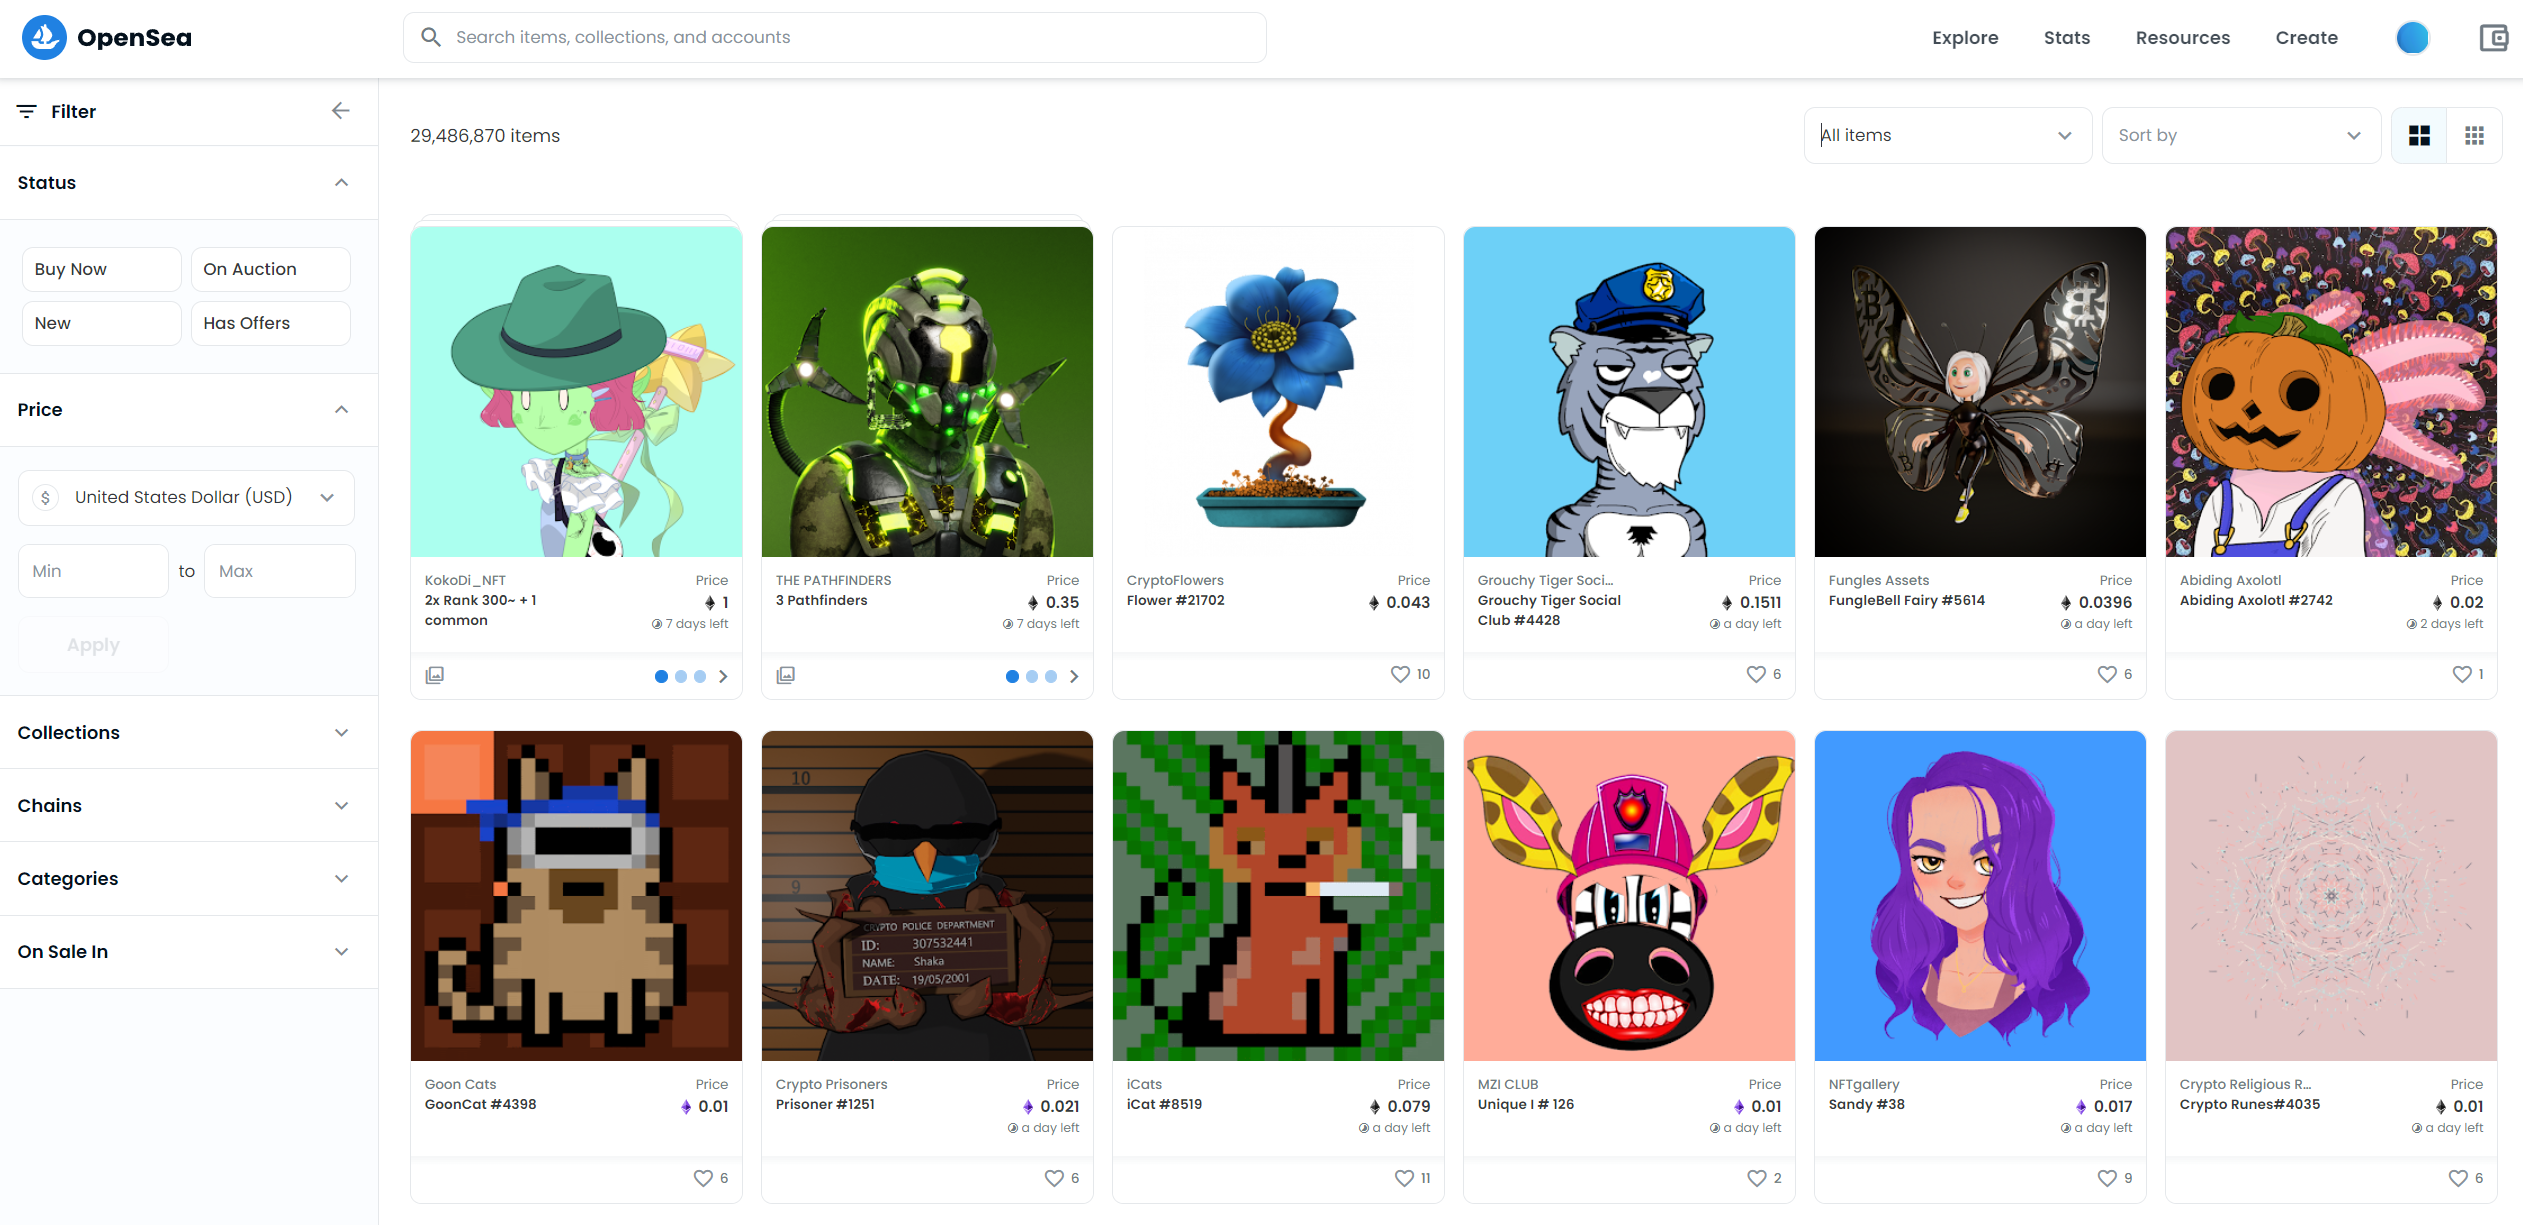
\includegraphics[width=\textwidth]{pics/openseaexample.png}
\end{center}
\end{frame}	


\begin{frame}
\frametitle{Why Do People Buy NFTs?}

%\begin{center}
%
\includegraphics[width=0.75\textwidth]{screenshots/skynet.png}
%\end{center}
\bi
\m If you walked into my home and saw the Mona Lisa hanging on my wall, what would you think? \pause 
\bi 
\m Could the cultural position of ``The Mona Lisa'' have been occupied by a different physical object? (I would say ``obviously yes'' -- we are in one of \textbf{multiple equilibria} possible) \pause 
\ei 
\m NFTs are ``art'', and also \ul{durable digital status goods}
\vspace{1ex}
\bi
\m Verifiably signals wealth (if market price is high!)
\vspace{1ex}
\m Private chat groups for NFT owners
\vspace{1ex}
\m Some convey rights/powers within videogames or virtual ``metaverse'' worlds
\ei
\vspace{1ex}
\m Explosive right-tail of returns attract speculative investors (``flippers'') 
\ei
	
\end{frame}


\begin{frame}
\frametitle{Strong cyclicality in volume}

\begin{center}
	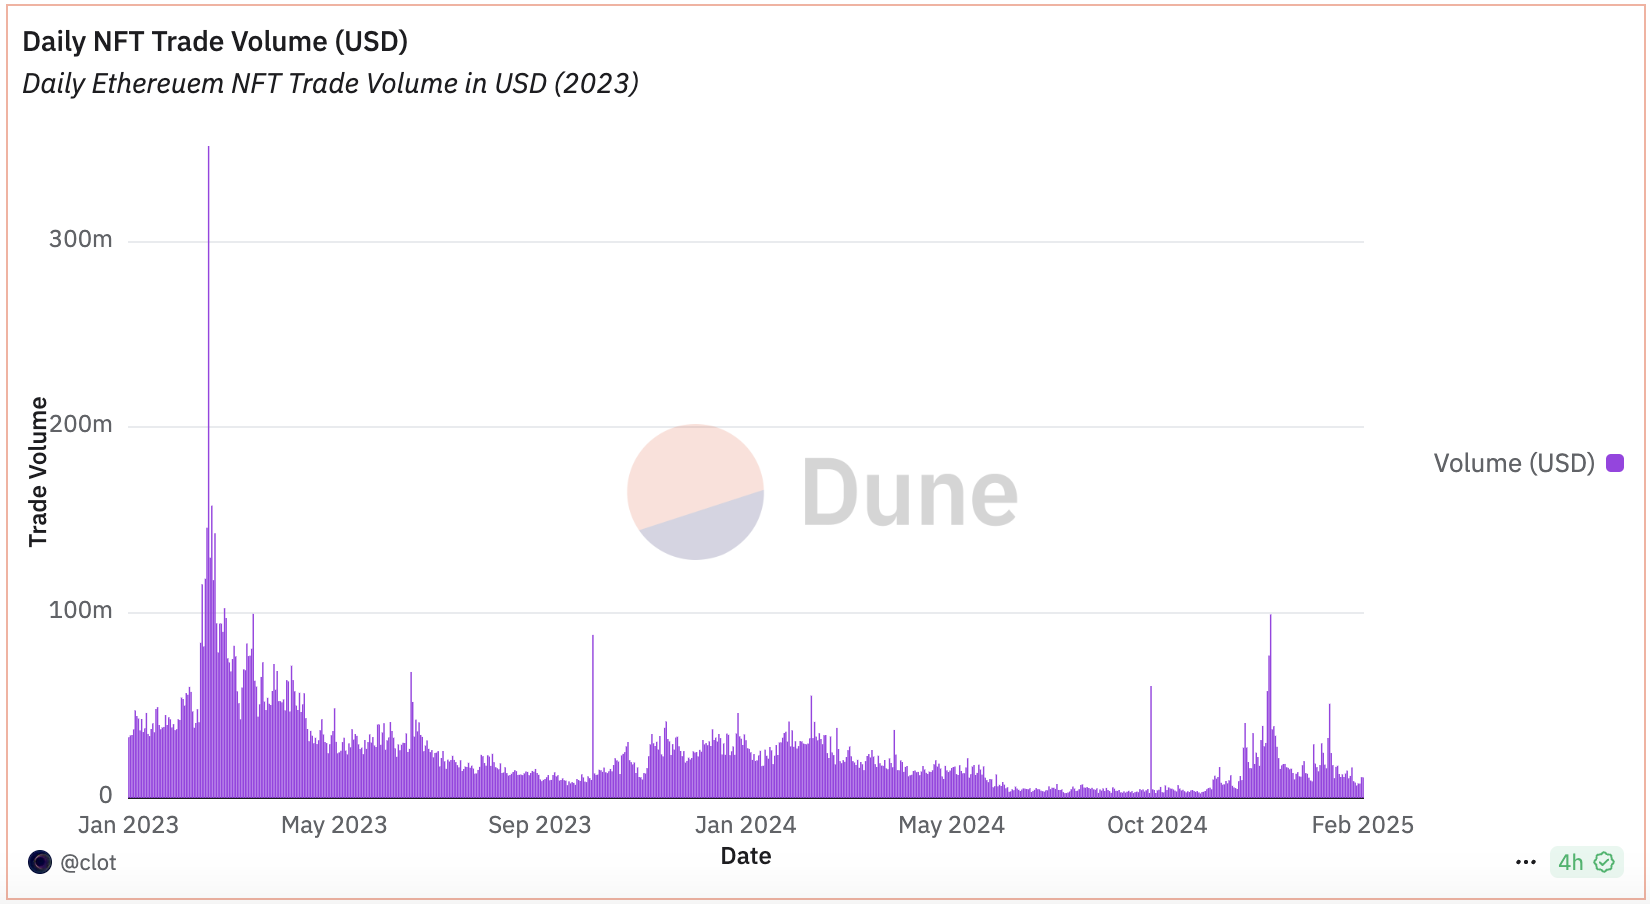
\includegraphics[width=0.9\textwidth]{Screenshot 2025-02-13 at 4.49.25 PM.png}
\end{center}

\href{https://dune.com/queries/2343578/3837381}{(Source)} ``One day you're in, the next day you're out.'' -Heidi Klum

\end{frame}

%\section{Veblen Goods}

%\begin{frame}
%\frametitle{Digital Veblen Goods (Oh, Rosen, Zhang 2023)}

%\bi
%\m NFTs as ``Veblen'' goods $\Longrightarrow$ a large social aspect to their value
%\m Key empirical findings confirming model predictions:
%\bi 
%\m NFT primary market outcomes are strikingly bimodal
%\m NFTs are systematically underpriced in primary markets (``mint premium'')
%\m ``Scalpers'' exploit issuers' pricing strategies to systematically extract profits% from the mint premium
%\ei 
%\ei

%\end{frame}


%\begin{frame}

%\begin{center}
%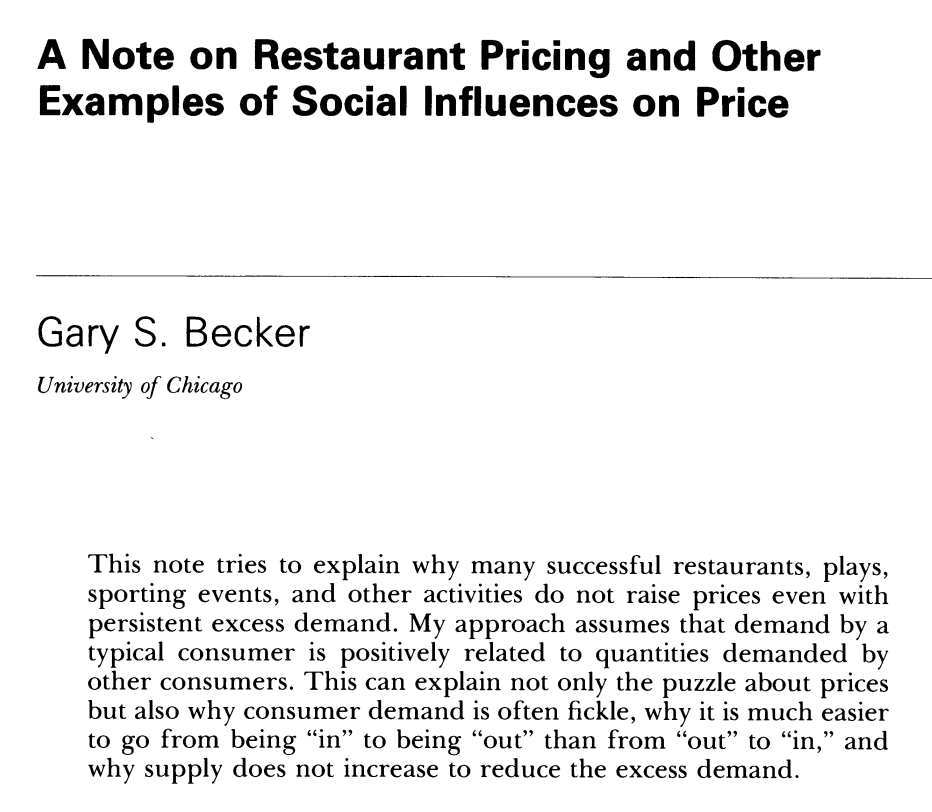
\includegraphics[width=0.7\textwidth]{pics/beckerrestaurants.png}
%\end{center}

%\end{frame}

\begin{frame}
\frametitle{Bank Runs and other ``Strategic Complementarities'' in Economics and Finance}

\bi
\m Recall how bank runs work:
\bi
\m If no one withdraws, everything is good. If everyone withdraws, the bank is insolvent
\m Diamond: ``Fear of fear itself''. Fear is a \ul{self-fulfilling prophecy}: if everyone thinks everyone else will withdraw, everyone wants to withdraw 
\ei
\m ``Social goods'' are similar -- but in reverse!
\bi
\m If nobody buys bored apes, they're uncool, and nobody wants to buy them
\m If everyone buys, I want to buy too! \ul{Demand begets demand}! 
\m Here, \ul{success} is a self-fulfilling prophecy: if everyone thinks everyone else will buy, everyone will buy\ldots
\ei
\ei

\end{frame}

\begin{frame}
\frametitle{Aside: ``Strategic Complementarities'' in Economics and Finance}

\bi
\m \ul{Markets}, generically, are settings with \ul{strategic substitutes}
\bi
\m When lots of people want to ski, ticket prices go up, so I'm less likely to ski
\m When lots of people study finance, wages go down\ldots
\ei
\m Substitutes naturally lead to \ul{unique equilibria} \pause
\m Bank runs, and social goods, display \ul{strategic complementarity}
\bi
\m When everyone withdraws, I want to withdraw
\m When everyone buys an NFT/Hermes bag/Rolex, it's cool and I want one too
\ei\pause
\m Strategic complementarities lead to \ul{multiple equilibria}
\bi
\m Banks with equal fundamentals can be solvent, or run on
%\m ``A Rolex by any other name\ldots''
\ei \pause
\m What are other examples of strategic complementarities? \pause
\m Is blockchain adoption, on the whole, more strategic substitutes or complements? Why?
\ei

\end{frame}

%\begin{frame}
%\frametitle{Testing the Social Goods Hypothesis}

%How would we test the hypothesis that ``social effects'' are important in NFT markets?
%\be
%\m \textbf{Bimodal outcomes} 
%\bi
%\m With social effects, something can be ``in'' or ``out'', but not in-between
%\m We should see collections either sell very well, or very poorly, but few in between!
%\ei \pause
%\m \textbf{Underpricing in primary markets} 
%\bi
%\m With social effects, demand is \ul{fragile}: if an ``in'' collection collapses to ``out'', it'll go from crowded to empty!
%\m Hermes/Rolex purposefully sets prices ``too low'', so items are ``overdemanded'' in primary markets
%\m This is never optimal if there aren't social effects
%\ei \pause
%\m \textbf{Scalping}
%\bi
%\m Due to underpricing, even if you don't want an Hermes bag, if you get one at retail, you can flip it for profits
%\m If we see underpricing, we should also see ``scalpers'' try to exploit issuers' underpricing
%\ei 

%\ee

%\end{frame}

\section{Equity Tokens and Governance}


\begin{frame}
\frametitle{Equity Issuance in Tradfi}

\bi
\m How do defi protocols issue ``equity''? How do they decide how to distribute to users? \pause
\m In tradfi, equity issuance is hard!
\bi
\m Public markets (publicly listed firms): harsh disclosure requirements, SEC scrutinizes every detail, new filings every quarter and for every issuance or ``material event'', etc. 
\m Private markets: limited to accredited investors, low liquidity  
\ei 
\m Recall that equity is traditionally bundled with control rights 
\bi 
\m This is negotiable, e.g. with \href{https://www.sciencedirect.com/science/article/pii/S0304405X21005407}{dual-class shares}
\m Why are these traditionally bundled together? \pause 
\m Equity-holders get the ``residual'' payouts after debt is paid, so payouts are highly sensitive to management decisions (unlike debt) 
\ei
\ei
\end{frame}

\begin{frame}
\frametitle{Equity Issuance in Defi}

\bi
\m ``Equity-like'' issuance in Defi is conceptually simple (if legally murky) 
\bi
\m Issue a ERC20 token
\m Write the governance and cash flow rights into the Solidity code 
\ei
\m Another big benefit over tradfi: issuers can target equity drops based on certain things, like usage, which is on-chain \pause 
\m Is this legal? \pause 
\bi 
\m Hard to argue an equity token is not an ``investment of money in a common enterprise with a reasonable expectation of profits to be derived from the efforts of others'' (The \href{https://www.sec.gov/about/divisions-offices/division-corporation-finance/framework-investment-contract-analysis-digital-assets}{Howey Test}) 
\ei 
\m Should it be? \pause 
\bi 
\m \textbf{Prosecutorial discretion} means government can unilaterally decline to prosecute crimes (e.g. DACA, FCPA, RIP CFPB) 
\ei 
\ei


\end{frame}


\begin{frame}
\frametitle{Tokens and Voting}

\bi
\m Tokens are a \ul{bundle} of rights:
\bi
\m Monetary (Sell token for \$\$\$!)
\m Utility (ETH used to pay gas)
\m Governance (MKR, UNI, CRV used to vote)
\ei
\m Not everyone values all rights! 
\m Voting rights can be lent and borrowed with flash loans 
\m When you \textbf{stake} your Proof-of-Stake crypto with a protocol like \href{https://polkadot.com/}{Polkadot}, you are trading them your voting rights in exchange for yield 
\ei

\end{frame}

\begin{frame}
\frametitle{A Diversion on Social Choice Theory}

\bi
\m Set of \textbf{outcomes:} Applebees $A$, Burger King $B$, Chipotle $C$ \pause
\m $1\ldots N$ people with \textbf{preferences}:
\bi
\m 1: $A>C>B$
\m 2: $A>C>B$
\m 3: $C>B>A$
\m 4: $B>C>A$
\ei \pause
\m A \ul{social choice function} maps preferences $\rightarrow$ outcomes \pause
\m Examples of social choice functions? \pause
\bi
\m \textbf{Plurality:} pick the most popular favorite (A) \pause
\m \textbf{Scoring rules:} make the least people choose their least favorite (C) \pause
\m \textbf{Dictatorship:} person 4 chooses (B)
\ei
\ei

\end{frame}

\begin{frame}
\frametitle{Arrow's Impossibility Theorem}

\bi
\m Set of \textbf{outcomes:} Applebees $A$, Burger King $B$, Chipotle $C$ \pause
\m Three good properties:
\be
\m \textbf{Pareto Efficiency:} If everyone prefers A to B, A chosen over B
\m \textbf{Independence of Irrelevant Alternatives:} Whether A chosen over B doesn't depend on how people rank $C$
\m \textbf{Non-Dictatorship:} choices aren't made by just one person!
\ee \pause
\m \textbf{Arrow's Impossibility Theorem:} no social choice rule satisfies all three properties at once! \pause
\m \textbf{Condorcet's Paradox} is the special case of AIT where ``cycles'' emerge a-la Rock-Paper-Scissors and no choice is stable 
\ei

\end{frame}

\begin{frame}
\frametitle{The Gibbard-Satterthwaite Theorem}

\bi
\m Arrow's theorem already assumes we know everyone's preferences! How do we elicit people to report their preferences? \pause
\m \textbf{Gibbard-Satterthwaite Theorem:} any voting rule which is non-dictatorial, and has more than two outcomes, is subject to \ul{strategic voting}
\bi
\m Someone has an incentive to vote ``untruthfully'' to influence outcomes
\ei \pause
\m What does strategic voting look like?
\bi
\m I like Applebee's but no one else does, so I'll pretend I like Burger King more than Applebee's, because it has a higher chance of winning
\ei \pause
\m This is true for \textbf{any nontrivial voting rule you use!}
\ei

\end{frame}


\begin{frame}
\frametitle{Social Choice Theory: Summary}

\bi
\m First and Second Welfare Theorems (Econ 101) prove that competitive markets can reach ``Pareto efficient'' outcomes under reasonable assumptions 
\pause
\m Social choice, however, is very hard! 
\bi
\m We can \ul{prove} that there are no ``good'' mechanisms!
\m Can only make tradeoffs among different kinds of ``bad'' 
\m \href{https://www.equal.vote/minimax}{Condorcet Methods} are a family of algorithms to minimize the extent of these ``bad'' properties 
\ei
\ei

\end{frame}

\begin{frame}
\frametitle{Shareholder Voting?}

\bi
\m Social choice in country settings is hard: we see many voting mechanisms in practice
\m But we generally see less arguments about shareholder voting: why? \pause
\m Anthony Zhang argues that shareholders'  \href{https://anthonyleezhang.substack.com/p/shareholder-voting-and-social-choice}{incentives are aligned} (recall the no-trade theorem!) 
\m Shareholder voting in a for-profit organization is an easier problem than social choice, because \textbf{we all want to maximize profits} \pause
\m We might disagree on the best business strategy to maximize profits, hence we need voting\ldots \pause
\ei


\end{frame}

%\begin{frame}
%\frametitle{What if we don't just care about money?}

%\begin{center}
%\includegraphics<1>[width=.7\textwidth]{pics/solarcity1.png}
%\includegraphics<2>[width=.6\textwidth]{pics/solarcity2.png}
%\end{center}

%\href{https://www.washingtonpost.com/technology/2022/04/27/musk-solarcity-verdict/}{Source}

%\end{frame}


\section{Airdrops}

\begin{frame}
\frametitle{Sushiswap ``Vampire Attack''}

\bi
\m 28 Aug 2020: Sushiswap launches, ``forked'' (copied open-source!) uniswap code
\m Same functionality as UNI - but \href{https://www.gemini.com/cryptopedia/sushiswap-uniswap-vampire-attack}{pays liquidity providers more and gives them governance rights} 
\bi
\m New SUSHI token paid to Uniswap Liquidity Providers who ``stake'' tokens with Sushi, has governance rights, and gets revenue from SUSHI trade fees
\ei
\m Then, a ``migration contract'' converts Uniswap LP tokens into Sushiswap LP tokens
\m \href{https://finematics.com/vampire-attack-sushiswap-explained/}{\$150mil} migrated within hours! Stole over 50\% of Uniswap's liquidity!
\ei
\end{frame}


\begin{frame}
\frametitle{The Uniswap Airdrop}

\bi
\m In response, on \href{https://uniswap.org/blog/uni}{September 16, 2020}, Uniswap announces launch of governance token, UNI. 60\% tokens reserved for ``community'' (users)
\m 15\% of total supply distributed retroactively to Uniswap users!
\m Airdropped \ul{minimum} \href{https://www.coindesk.com/markets/2020/09/17/uniswap-recaptures-defi-buzz-with-uni-tokens-airdropped-debut/}{400\$UNI} \textbf{per user}, worth over \$1000 USD!
\bi 
\m An \textbf{Airdrop} is a strategy where crypto developers issue tokens for free to certain wallets to try to jump-start a user base (or in this case, win it back)
\ei 
\m 45\% reserved for future user incentives
\ei

\end{frame}

\begin{frame}
\frametitle{Sushiswap and Uniswap}

\begin{center}
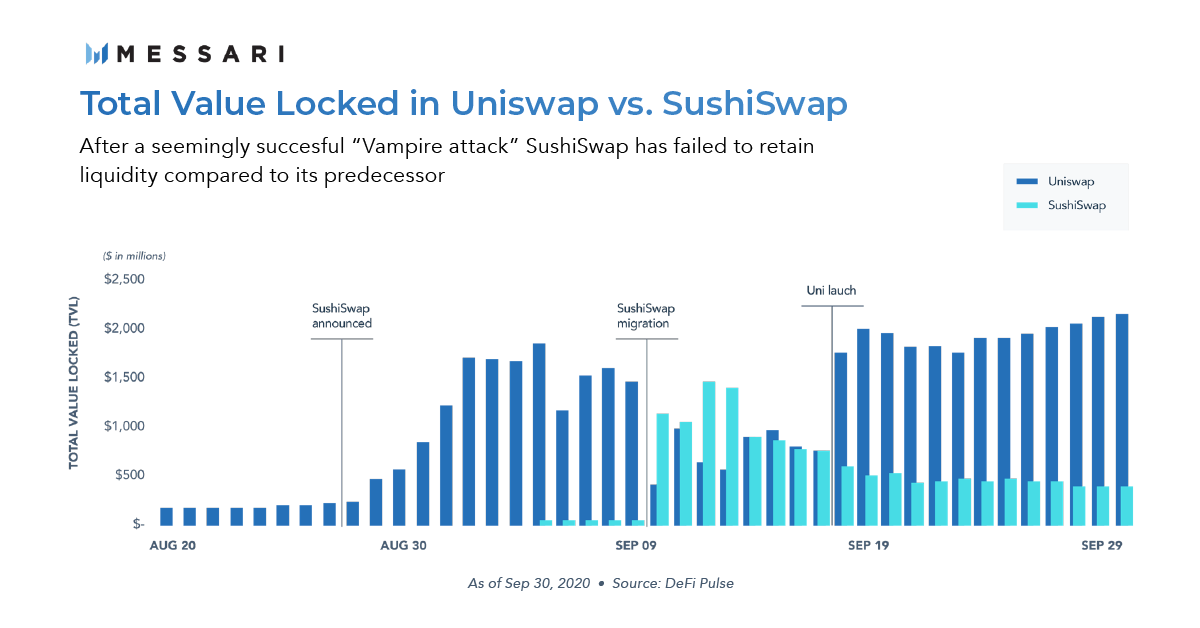
\includegraphics[width=\textwidth]{pics/sushi.png}
\end{center}

\footnotesize
\href{https://twitter.com/MessariCrypto/status/1318229445581430798}{Source}
\end{frame}


\begin{frame}
\frametitle{Sushiswap and Uniswap}

\bi
\m Moral of Sushi/Uniswap saga?
\ei \pause

\bi
\m If you don't give users equity (+governance), we'll clone you and add an equity (+governance) token, and beat you \pause 
\m I must ask, again, is this legal? \pause 
\m SEC, April 10, 2014: \href{https://gov.uniswap.org/t/the-uni-token-and-its-future/16044/4}{No} \pause 
\m Trump-apppointed SEC commissioner Mark Uyeda will decide whether to continue to pursue the case, or exercise prosecutorial discretion. 
\ei

\end{frame}

\begin{frame}
\frametitle{The Airdrop Sybil Wars}

\bi
\m \$UNI airdrop was a surprise! But soon started a trend...
\m Airdrops are often not directly proportional to ownership (why?) \pause
\bi
\m Want token distribution to be more ``democratic'', not too much whale control
\ei \pause
\m But if they give you one airdrop per wallet... \pause Make more wallets!
\m Referred to as a \textbf{Sybil attack} after a book about multiple personality disorder 
\ei

\begin{center}

\includegraphics[width=0.2\textwidth]{pics/sybil.jpeg}
\end{center}

\end{frame}



\begin{frame}
\frametitle{The Airdrop Sybil Wars: Ribbon Finance}

\bi
\m \href{https://www.ribbon.finance/}{Ribbon Finance}, a structured products protocol, did a retroactive airdrop in Oct 2021
\m Ribbon told VC Divergence Ventures, which invested \$25k in Ribbon, about the upcoming airdrop
\m A Divergence Ventures analyst then made a huge number of wallets, making \$2.5mil from Sybil attacking the airdrop!
\m \href{https://twitter.com/gabagooldoteth/status/1446498569603756033}{People were not happy!} Divergence eventually \href{https://etherscan.io/tx/0xbdd294f2e43701f66a55499afcfa4db5385b6f88f44d3390519811ea072e35e0}{sent the ETH back to Ribbon}
\m Interesting lesson also about defi community culture and standards!
\ei

\vspace{0.4in}

\footnotesize
References: \href{https://www.coindesk.com/tech/2021/10/08/airdrop-ethics-vc-firm-draws-ire-following-25m-ribbon-finance-exploit/}{Coindesk} and \href{https://cryptobriefing.com/divergence-ventures-analyst-exposed-farming-airdrop/}{Crypto Briefing} articles

\end{frame}

\begin{frame}
\frametitle{The Airdrop Sybil Wars: Ribbon Finance}

\begin{center}
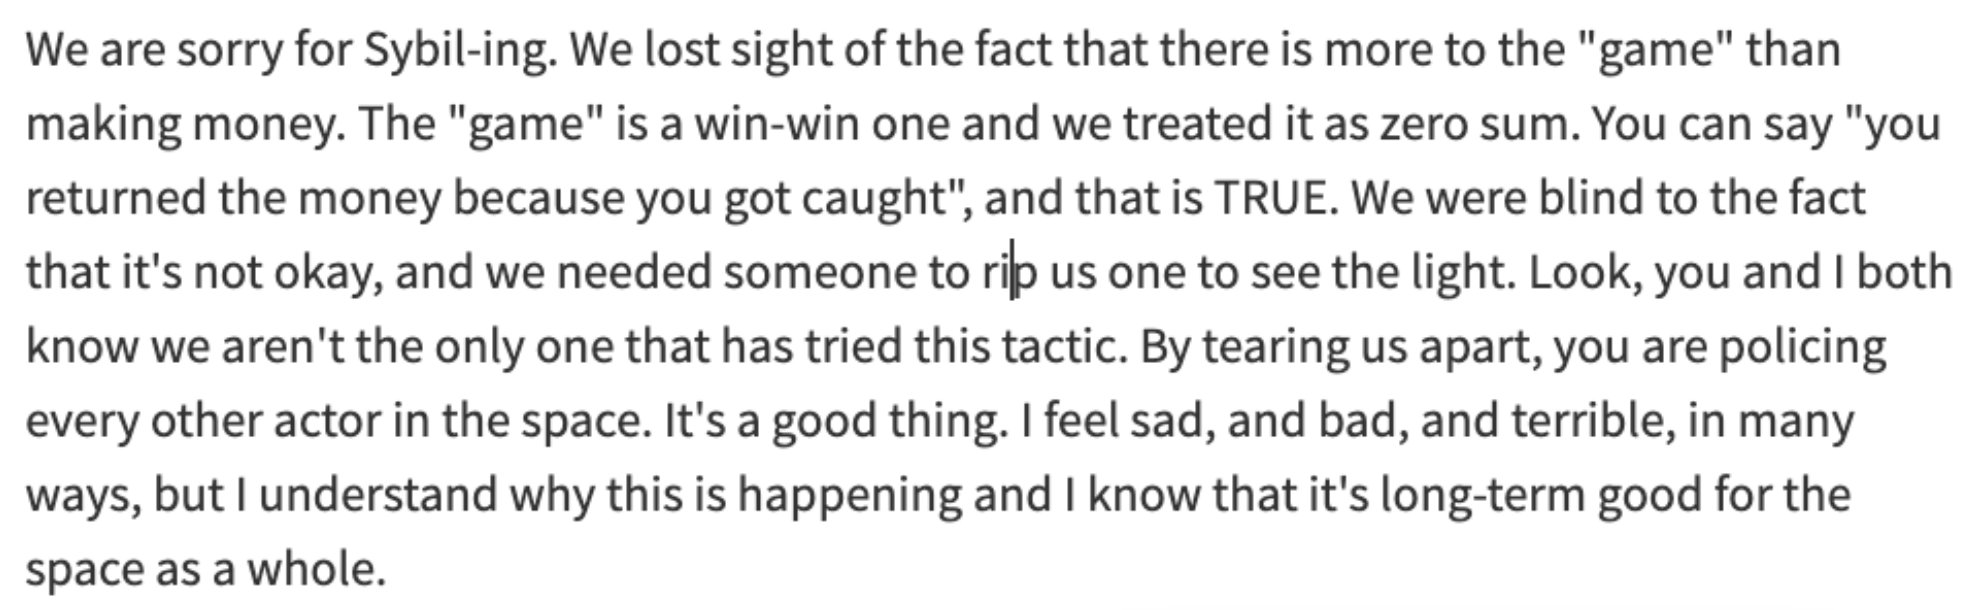
\includegraphics[width=\textwidth]{pics/sorry}
\end{center}

\end{frame}

\begin{frame}
\frametitle{The Airdrop Sybil Arms Race}

\small

\bi
\m Started an ``arms race'' between sybils attackers and airdroppers \pause
\m \href{https://medium.com/paraswap/introducing-the-psp-token-to-make-paraswap-even-more-efficient-and-decentralized-c4730e50be72}{Paraswap}, an AMM aggregator protocol, airdropped a token to only 1.5\% of users, applying \href{https://medium.com/paraswap/whats-an-active-user-clarifying-psp-token-distribution-filtering-logic-81df6096d410}{bespoke filters to screen out airdrop hunters} \pause
\m \href{https://hop.exchange/}{Hop protocol}, an ETH L2 exchange, even \href{https://twitter.com/HopProtocol/status/1522284558179307522}{paid people with tokens to help find Sybil attackers!} \pause
\m Regulatory risk: \href{https://dydx.exchange/}{dYdX}, a derivatives protocol, did a huge airdrop (Over \$50k USD some users!), but \href{https://www.coindesk.com/business/2021/09/08/users-celebrate-massive-dydx-token-airdrop-as-transfer-restrictions-lift/}{filtered out US IP addresses} 
\m Most airdrop projects have many anti-Sybil criteria now. 
%\m Long list of airdrops not mentioned: COMP, ENS, OP, 
%\m NFT airdrops: BAYC, Azuki, and others
\ei 

\end{frame}


\begin{frame}
\frametitle{Airdrops: technology}

\bi
\m Airdrops enabled by the possibility of targeted based on verified on-chain data
\m Imagine: see every thing a person ever bought, use this to target equity drops!
\m Across all company boundaries (SOS used Opensea data)
\bi
\m Marketing implications: free targeting your competitors!
\ei
\m Sybil attacks, defense, etc. 
\m No/low chance of "lost in mail"
\ei

\end{frame}

\begin{frame}
\frametitle{Governance responsibility, community}

\begin{center}
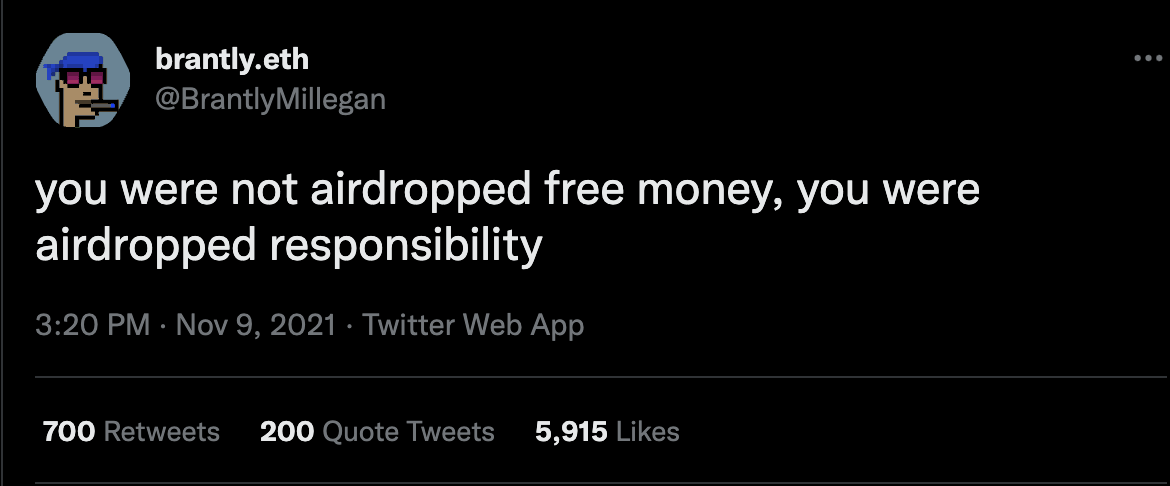
\includegraphics[width=\textwidth]{pics/responsibility}
\end{center}

\end{frame}


\begin{frame}
\frametitle{Aside: Vitalik, SHIB, and COVID India}

\bi
\m In 2021, was popular to launch dog meme coins, which had no purpose, but somehow still had value
\m Was popular to airdrop a large \% of meme coins to Vitalik Buterin, whose address is public
\m Vitalik faces a difficult problem!
\bi
\m Hodl coin? Tax implications, etc.?
\bi 
\m ``Hodl'' is crypto-speak for ``Hold'' (i.e. ``not sell'')
\ei 
\m Sell coin? Accused of dumping on retail? 
\ei 
\ei

\end{frame}

\begin{frame}{What to do with \$1B in Meme Coins?}

Vitalik's \href{https://etherscan.io/tx/0xb65bcbb85c1633b0ab4e4886c3cd8eeaeb63edbb39cacdb9223fdcf4454fd2c7}{solution}: 

\begin{center}

\includegraphics[width=0.8\textwidth]{pics/shib}
\end{center}  

\end{frame}


\end{document}